\documentclass[border=1mm, convert = false]{standalone}
\usepackage{amsmath, amssymb, amsfonts}
\usepackage{tikz}
\usepackage{helvet}
\renewcommand{\familydefault}{\sfdefault}

\begin{document}

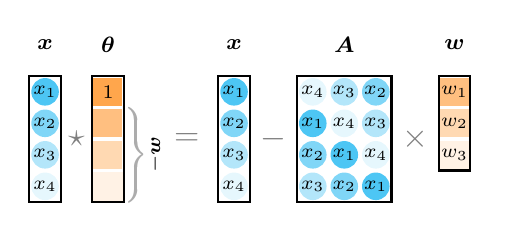
\begin{tikzpicture}[domain=0:4]
    \newcommand{\posx}{4}
    \newcommand{\posy}{3.8}

    \draw [step=0.4, very thick, color=white] (0+0.8,0.4-4) grid (0.4+0.8,2-4);
    \draw [thick] (0+0.8,0.4-4) rectangle (0.4+0.8,2-4);
    \draw (1,3-4-0.6) node {\footnotesize{\color{black}$\boldsymbol{x}$}};
    \node[circle,fill=cyan!70,inner sep=0pt,minimum size=0.35cm] at (1,1.8-4) {\scriptsize\color{black}$x_1$};
    \node[circle,fill=cyan!50,inner sep=0pt,minimum size=0.35cm] at (1,1.4-4) {\scriptsize\color{black}$x_2$};
    \node[circle,fill=cyan!30,inner sep=0pt,minimum size=0.35cm] at (1,1-4) {\scriptsize\color{black}$x_3$};
    \node[circle,fill=cyan!10,inner sep=0pt,minimum size=0.35cm] at (1,0.6-4) {\scriptsize\color{black}$x_4$};

    \draw (2-0.6,1.2-4) node {\large{\color{gray}$\star$}};
    
    \filldraw [fill=orange!70] (5.2-3.6,0.4-4) rectangle (5.6-3.6,2-4);
    \filldraw [fill=orange!50] (5.2-3.6,1.2-4) rectangle (5.6-3.6,1.6-4);
    \filldraw [fill=orange!30] (5.2-3.6,0.8-4) rectangle (5.6-3.6,1.2-4);
    \filldraw [fill=orange!10] (5.2-3.6,0.4-4) rectangle (5.6-3.6,0.8-4);
    \draw [step=0.4, very thick, color=white] (5.2-3.6,0.8-4) grid (5.6-3.6,2-4);
    \draw [thick] (5.2-3.6,0.4-4) rectangle (5.6-3.6,2-4);
    \draw (5.4-3.6,3-4-0.6) node {\footnotesize{\color{black}$\boldsymbol{\theta}$}};

    \draw (5.4-3.6,1.8-4) node {\scriptsize{\color{black}$1$}};
    \draw (5.4-3.6,1.4-4) node {};
    \draw (5.4-3.6,1.0-4) node {};
    \draw (5.4-3.6,0.6-4) node {};

    \draw (5.4-3.25,0.6-3.6) node[rotate = 90] {{\color{gray!65}$\underbrace{\hspace{1.2cm}}$}};
    \draw (5.4-3,0.6-3.6) node[rotate = 90] {\scriptsize{\color{black}$-\boldsymbol{w}$}};

    \draw (2-0.2+1,1.2-4) node {\large{\color{gray}$=$}};

    \draw [step=0.4, very thick, color=white] (0+0.8+2.4,0.4-4) grid (0.4+0.8+2.4,2-4);
    \draw [thick] (0+0.8+2.4,0.4-4) rectangle (0.4+0.8+2.4,2-4);
    \draw (1+2.4,3-4-0.6) node {\footnotesize{\color{black}$\boldsymbol{x}$}};
    \node[circle,fill=cyan!70,inner sep=0pt,minimum size=0.35cm] at (1+2.4,1.8-4) {\scriptsize\color{black}$x_1$};
    \node[circle,fill=cyan!50,inner sep=0pt,minimum size=0.35cm] at (1+2.4,1.4-4) {\scriptsize\color{black}$x_2$};
    \node[circle,fill=cyan!30,inner sep=0pt,minimum size=0.35cm] at (1+2.4,1-4) {\scriptsize\color{black}$x_3$};
    \node[circle,fill=cyan!10,inner sep=0pt,minimum size=0.35cm] at (1+2.4,0.6-4) {\scriptsize\color{black}$x_4$};

    \draw (4.5-0.6,1.2-4) node {\large{\color{gray}$-$}};

    \draw [step=0.4, very thick, color=white] (2.8-0.2+1.6,0.4-4) grid (4-0.2+1.6,2-4);
    \draw [thick] (2.8-0.2+1.6,0.4-4) rectangle (4-0.2+1.6,2-4);
    \draw (3.4-0.2+1.6,3-4-0.6) node {\footnotesize{\color{black}$\boldsymbol{A}$}};
    \node[circle,fill=cyan!10,inner sep=0pt,minimum size=0.35cm] at (3-0.2+1.6,1.8-4) {\scriptsize\color{black}$x_4$};
    \node[circle,fill=cyan!70,inner sep=0pt,minimum size=0.35cm] at (3-0.2+1.6,1.4-4) {\scriptsize\color{black}$x_1$};
    \node[circle,fill=cyan!50,inner sep=0pt,minimum size=0.35cm] at (3-0.2+1.6,1-4) {\scriptsize\color{black}$x_2$};
    \node[circle,fill=cyan!30,inner sep=0pt,minimum size=0.35cm] at (3-0.2+1.6,0.6-4) {\scriptsize\color{black}$x_3$};
    \node[circle,fill=cyan!30,inner sep=0pt,minimum size=0.35cm] at (3.4-0.2+1.6,1.8-4) {\scriptsize\color{black}$x_3$};
    \node[circle,fill=cyan!10,inner sep=0pt,minimum size=0.35cm] at (3.4-0.2+1.6,1.4-4) {\scriptsize\color{black}$x_4$};
    \node[circle,fill=cyan!70,inner sep=0pt,minimum size=0.35cm] at (3.4-0.2+1.6,1-4) {\scriptsize\color{black}$x_1$};
    \node[circle,fill=cyan!50,inner sep=0pt,minimum size=0.35cm] at (3.4-0.2+1.6,0.6-4) {\scriptsize\color{black}$x_2$};
    \node[circle,fill=cyan!50,inner sep=0pt,minimum size=0.35cm] at (3.8-0.2+1.6,1.8-4) {\scriptsize\color{black}$x_2$};
    \node[circle,fill=cyan!30,inner sep=0pt,minimum size=0.35cm] at (3.8-0.2+1.6,1.4-4) {\scriptsize\color{black}$x_3$};
    \node[circle,fill=cyan!10,inner sep=0pt,minimum size=0.35cm] at (3.8-0.2+1.6,1-4) {\scriptsize\color{black}$x_4$};
    \node[circle,fill=cyan!70,inner sep=0pt,minimum size=0.35cm] at (3.8-0.2+1.6,0.6-4) {\scriptsize\color{black}$x_1$};

    \draw (4.5+1.2,1.2-4) node {\large{\color{gray}$\times$}};
    
    \filldraw [fill=orange!50] (5.2+0.8,0.8-4) rectangle (5.6+0.8,2-4);
    \filldraw [fill=orange!30] (5.2+0.8,1.2-4) rectangle (5.6+0.8,1.6-4);
    \filldraw [fill=orange!10] (5.2+0.8,0.8-4) rectangle (5.6+0.8,1.2-4);
    \draw [step=0.4, very thick, color=white] (5.2+0.8,0.8-4) grid (5.6+0.8,2-4);
    \draw [thick] (5.2+0.8,0.8-4) rectangle (5.6+0.8,2-4);
    \draw (5.4+0.8,3-4-0.6) node {\footnotesize{\color{black}$\boldsymbol{w}$}};

    \draw (5.4+0.8,1.8-4) node {\scriptsize{\color{black}$w_1$}};
    \draw (5.4+0.8,1.4-4) node {\scriptsize{\color{black}$w_2$}};
    \draw (5.4+0.8,1.0-4) node {\scriptsize{\color{black}$w_3$}};

\end{tikzpicture}

\end{document}